\documentclass[a4paper, 14pt]{article}
\usepackage[utf8]{inputenc}
\usepackage[russian]{babel}
\usepackage{graphicx}
\usepackage{hyperref}


\usepackage{listings}
\lstset{
	language=C++,
	numbers=left,
	frame=single,
	breaklines=true,
	breakatwhitespace=true,
	title=lstname,
	tabsize=4	
}

\usepackage{color}
\usepackage{amsmath}
\usepackage{pgfplots}
\usepackage{url}

\usepackage{titlesec}
\titleformat*{\section}{\LARGE\bfseries}
\titleformat*{\subsection}{\Large\bfseries}
\titleformat*{\subsubsection}{\large\bfseries}
\titleformat*{\paragraph}{\large\bfseries}
\titleformat*{\subparagraph}{\large\bfseries}

\begin{document}
	\begin{titlepage}
		\begin{center}
			\begin{LARGE}
				Отчет по лабораторной работе №1\\
				по курсу "Анализ алгоритмов"\\
				по теме "Расстояние Левенштейна"
			\end{LARGE}
			
			\begin{Large}
				\vspace{10cm}
				Студент: Барсуков Н.М. ИУ7-56\\
				Преподаватель: Волкова Л.Л.,
				Строганов Ю.В.
			\end{Large}
		\end{center}
	\end{titlepage}

	\tableofcontents
	
	\newpage
	\section*{Введение}
	
	Расстояние Левенштейна (также редакционное расстояние или дистанция редактирования) между двумя последовательностями символов.  В теории информации и компьютерной лингвистике — это минимальное количество операций вставки одного символа, удаления одного символа и замены одного символа на другой, необходимых для превращения одной строки в другую.\\
	
	Расстояние Левенштейна и его обобщения активно применяются \cite{primenenie}:
	
	\begin{enumerate}
		\item для исправления ошибок в слове (в поисковых системах, базы данных, при вводе текста, при автоматическом распознавании отсканированного текста и речи);
		\item в биоинформатике для сравнения генов, хромосом, белков.
	\end{enumerate}
	
	\newpage
	\section{Аналитическая часть}
	
	Цель: Изучить, реализовать и сравнить алгоритмы вычисления редакционного расстояния между 2 строками
	
	Для этого необходимо выполнить следующие пункты:
	
	\begin{enumerate}
		\item Иследовать алгоритмы вычисления редакционного расстояния;
		\item Реализовать следующие алгоритмы:
		\begin{enumerate}
			\item Итеративный;
			\item Рекурсивный;
			\item Модифицированный итеративный.
		\end{enumerate}
		\item Сделать замеры выбранных алгоритмов;
		\item Сравнить результаты замеров;
		\item Сделать вывод.
	\end{enumerate}
	
	\vspace{5mm}
	В нашей лабораторной работе будет рассматриваться 2 способа реализации данного алгоритма.
	
	\begin{enumerate}
		\item Итеративный;
		\item Рекурсивный.
	\end{enumerate}
		
	\vspace{5mm}
	Все они работает по следующему принципу. Допустим,что существует две строки S1 и S2 над некоторым алфавитом. Длина одной из них - M, второй - N. Для нахождения расстояния Левенштейна между ними D(S1, S2) можно применить следующую формулу (D(S1, S2) == D(M, N))\cite{primenenie}  (\ref{for1}  \ref{for2}):

		\begin{equation}\label{for1}
			D(i,j)=\begin{cases}
			max(i,j)\ if\ min(i,j) == 0\\
			min\begin{cases}
			D(i,j-1) + 1\\
			D(i-1,j) + 1\\
			D(i-1,j-1) + (S1[i] <> S2[j])
			\end{cases}
			\end{cases}
		\end{equation} 
		

		\begin{equation}
			D(i,j)=\begin{cases}
			max(i,j)\ if\ min(i,j) == 0\\
			min\begin{cases}
			D(i,j-1) + 1\\
			D(i-1,j) + 1\\
			D(i-1,j-1) + (S1[i] <> S2[j])\\
			D(i-2,j-2) + 1
			\end{cases} \ if \ i,j>1\\
			min\begin{cases}
			D(i,j-1) + 1\\
			D(i-1,j) + 1\\
			D(i-1,j-1) + (S1[i] <> S2[j])
			\end{cases}
			\end{cases}
			\label{for2}					
			\end{equation}

	\vspace{5mm}
	
	Так же вводится понятие стоимости операций. По умолчанию предполагается, что каждая операция, кроме операции сравнения символом, стоят по 1. Введем собственную стоимость для нашего случая:

	\begin{enumerate}
		\item Вставка в S1 (I) - 1;
		\item Удаление из S1 (D) - 1;
		\item Замена символа в S1 (R) - 1;
		\item Обмен местами 2 соседних символов (S) - 1;
		\item Совпадение символов в S1 и S2 - 0.
	\end{enumerate}

	\subsubsection{Вывод}
	
	В данном разделе были рассмотрены алгоритмы поиска редакционного расстояния Левенштейн и Левенштейн - Дамерау, который является модифицированной версией первого и вводит дополнительную операцию перестановки двух ближних символов 
	
	Мы будем рализовывать 2 
	
	\newpage
	\section{Конструкторский раздел}
	
	В данном разделе буду приведены блок схемы и описана структура программы
	
	\subsection{Алгоритм}
	
	В данном подразделе буду представлены схемы итеративного(\ref{fig:unnamed1}), рекурсивного(\ref{fig:1}), модифицированного алгоритма(\ref{fig:2}). Как вы можете заметить схема отличается только дополнительной проверкой и введением дополнительной операции.
	
	
	\begin{figure}[!h]
		\centering
		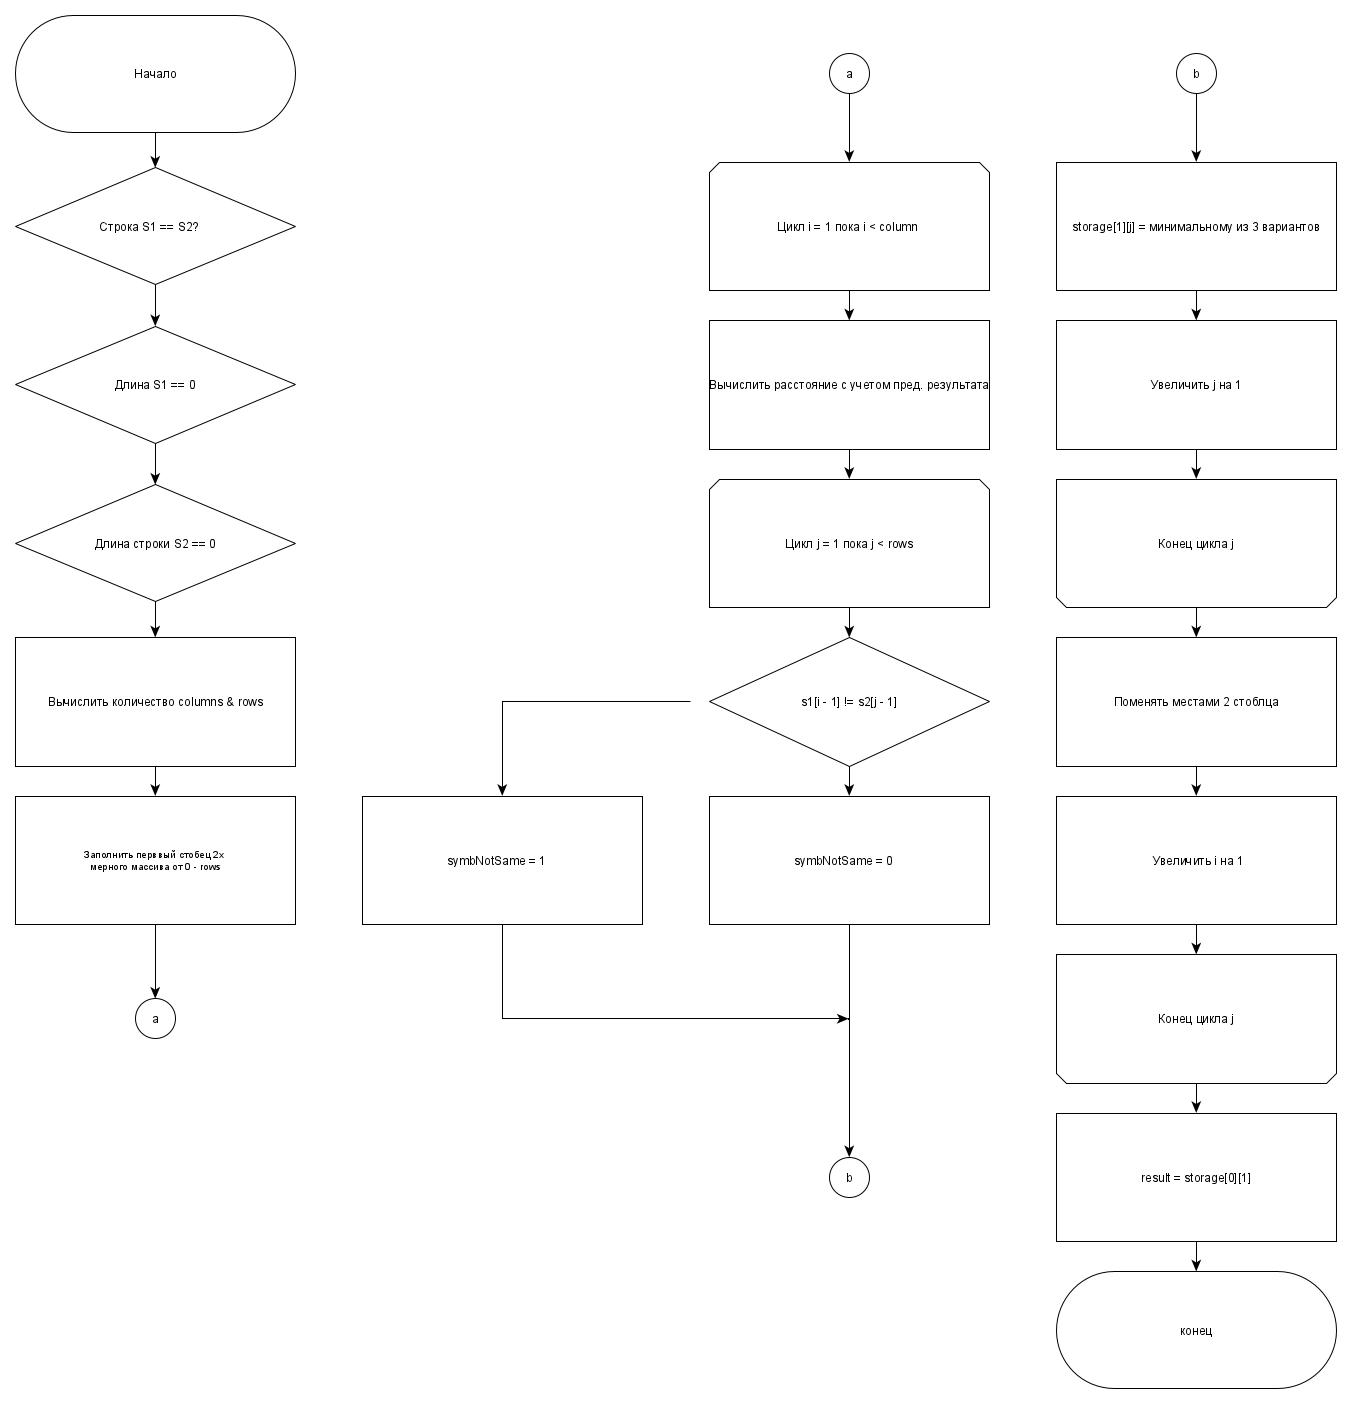
\includegraphics[width=0.7\linewidth]{img/unnamed1}
		\caption{Схема итеративного алгоритма}
		\label{fig:unnamed1}
	\end{figure}
	
	\newpage
	\begin{figure}[!h]
		\centering
		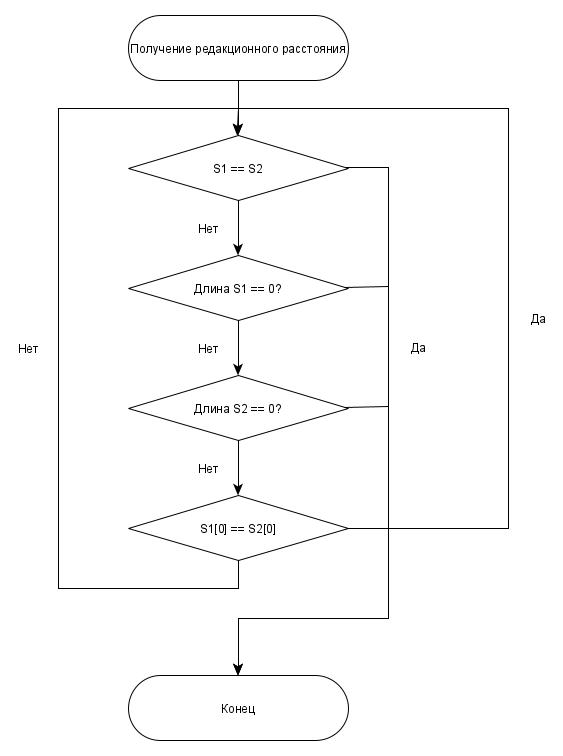
\includegraphics[scale=0.5]{img/1}
		\caption{Блок схема рекурсивного алгоритма}
		\label{fig:1}
	\end{figure}

	\begin{figure}[!h]
		\centering
		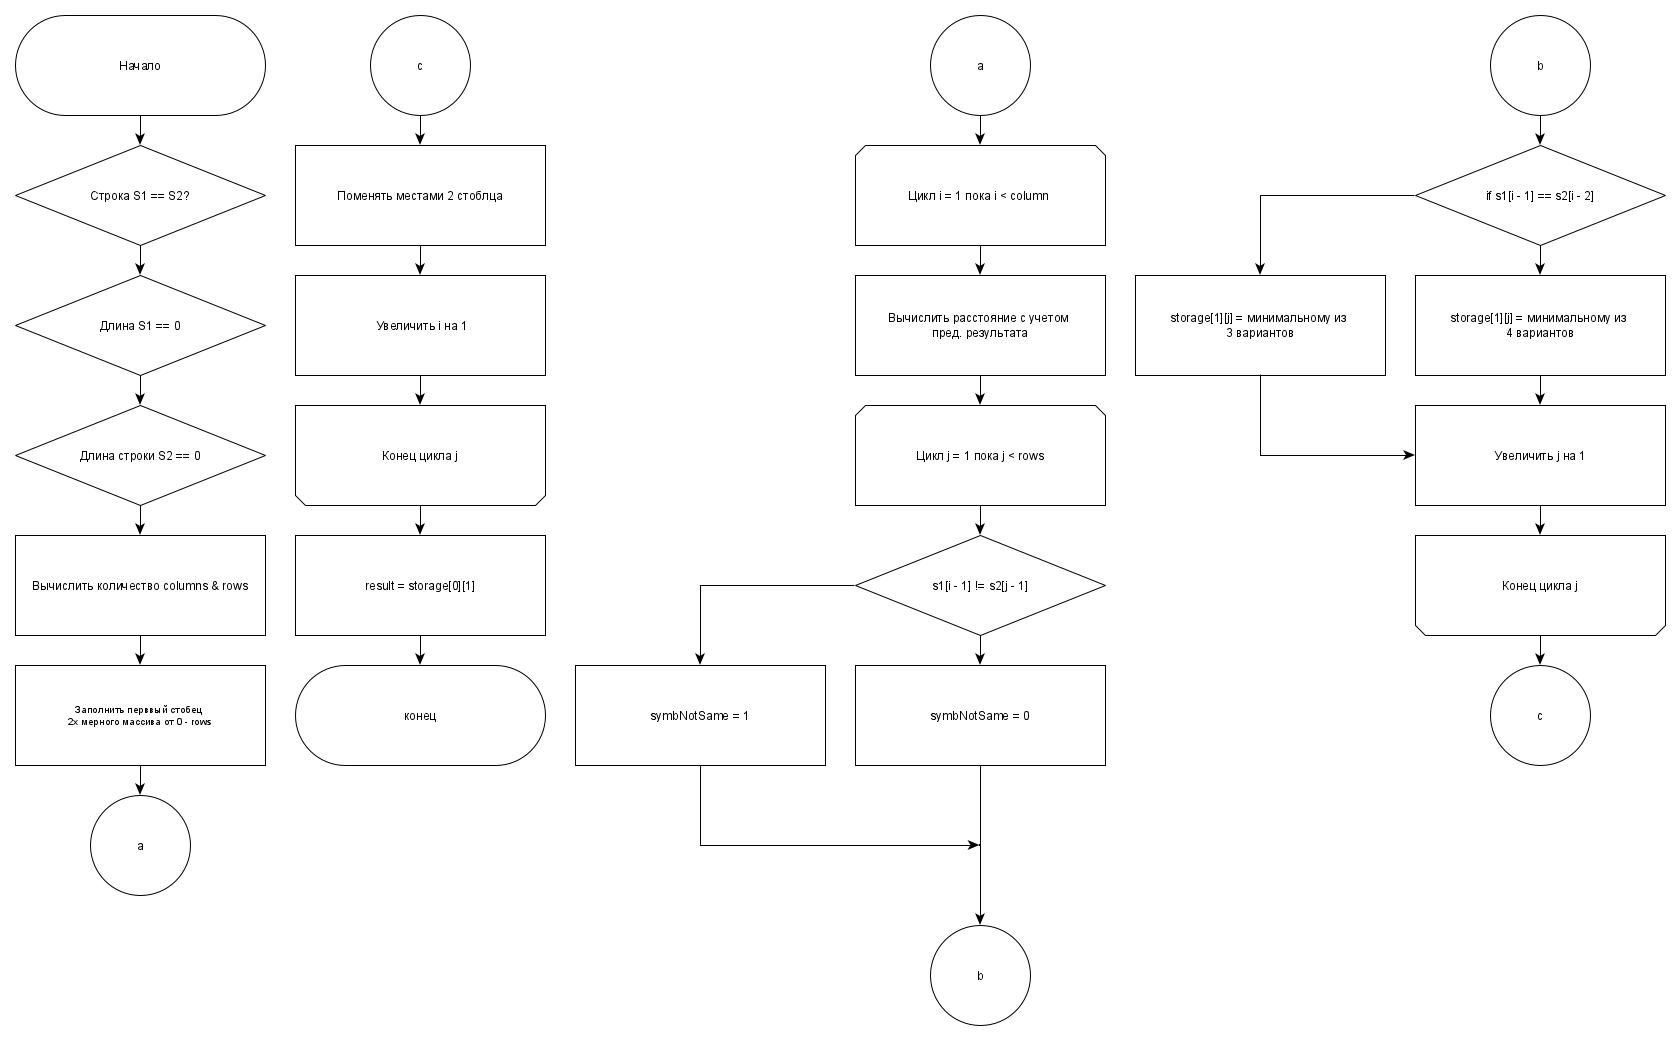
\includegraphics[width=0.7\linewidth]{graph/2}
		\caption{Блок схема мод. алгоритма}
		\label{fig:2}
	\end{figure}
	
	

	\subsection{Структура программы}
	
	Программа обладает следующей структурой:
	
	\begin{enumerate}
		\item приветственное окно в котором пользоваетелся знакомят с программой и просят выбрать режим работы. Режимы следующие:
		\begin{enumerate}
			\item поиск редакционного расстояния на 2 строках введенных пользователем;
			\item поиска редакционного расстояния на случайных строках длины указанной пользователем.
		\end{enumerate}
	\end{enumerate}

	\subsection{Вывод}
	В данном разделе были представлены схемы итеративного (матричного), рекурсивного и модифицированного Левенштейна и структура программы 
	
	\newpage
	\section{Технологический раздел}
	
	В данном разделе будут описаны требования к программному продукту и инструментарий реализации. Приведен интерфейс программы и листинг кодов алгоритмов
	
	\subsection{Требования}
	
	Требования к данному программному продукту следующие:
	\begin{enumerate}
		\item программа должна корректно работать;
		\item возвращать редакционное расстояние между 2 строк длинной до 10000 символов;
		\item не должна обрабатывать некорректный вод, ответственность ложиться на пользователя 
	\end{enumerate}

	\subsection{Выбор языка и среды разработки}
	
	Для решения данной поставленной задачи, мной был выбран язык с++ стандарта  \href{http://www.open-std.org/jtc1/sc22/wg14/www/docs/n1548.pdf}{c11} по причине использования структурного подхода и его мультиплатформенности.
	
	Так же мной используются среда разработки под названием \href{https://visualstudio.microsoft.com/ru/vs/}{Visual Studio 2019} по причине удобства отладки и функциональности. И так же желания изучить данную среду по лучше.
	
	\subsection{Интерфейс}
	
	Интерфейс представляет из себя простую консоль в котором пользователь взаимодействует с помощью ввода команд. Такой тип взаимодействия выбран, по причине простоты разработки и удобства тестирования программы (\ref{fig:screen1}, \ref{fig:screen2}).
	
	\begin{figure}[!h]
		\centering
		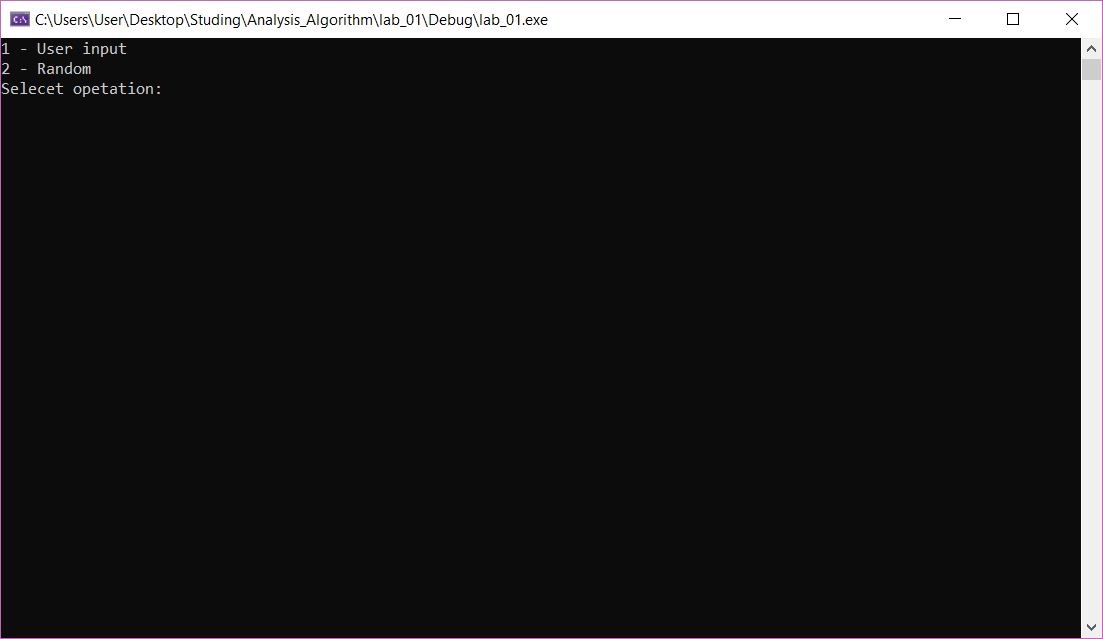
\includegraphics[width=0.7\linewidth]{img/screen1}
		\caption{Примера работы}
		\label{fig:screen1}
	\end{figure}
	
	\begin{figure}[!h]
		\centering
		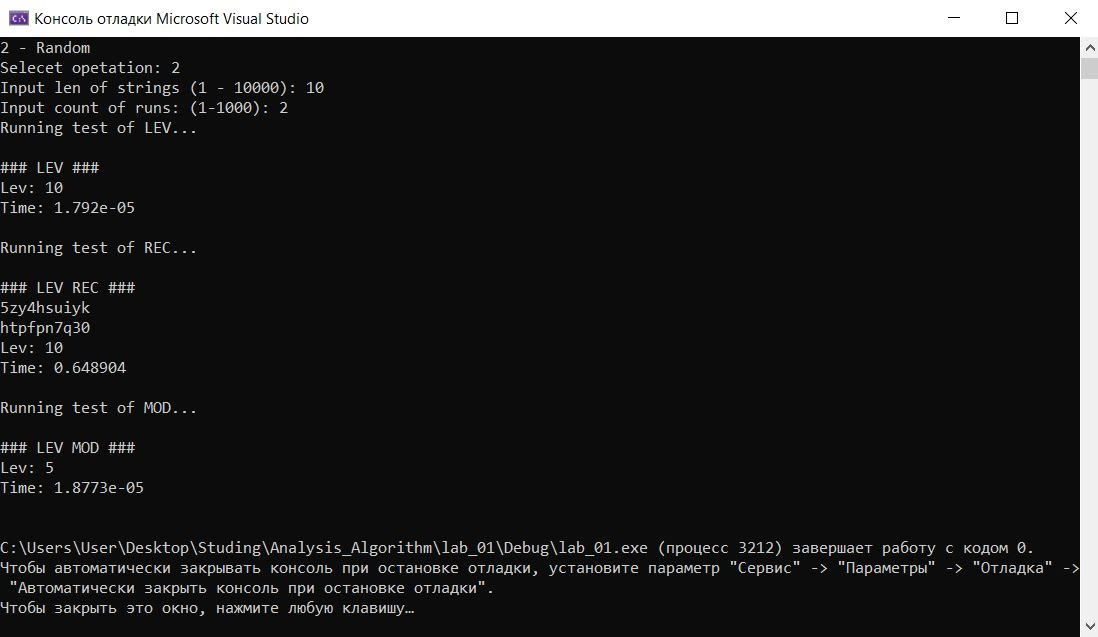
\includegraphics[width=0.7\linewidth]{img/screen2}
		\caption[]{Примера работы}
		\label{fig:screen2}
	\end{figure}
	
	
	\subsection{Листинг}
	Ниже будут представлены листинги итеративного (\ref{llevclass}), рекурсивного (\ref{llevrec}), модифицированного (\ref{llevmod})
	
	\lstinputlisting[firstline=10, lastline=56, caption= Итеративный алгоритм, label=llevclass]{Levenstain3.cpp}

	\vspace{5mm}
	
	\lstinputlisting[firstline=59, lastline=83, caption=Рекурсивный алгоритм, label=llevrec]{Levenstain3.cpp}
	
	\vspace{5mm}
	
	\lstinputlisting[firstline=10, lastline=75, caption=Левенштейн модифицированный, label=llevmod]{Levenstain4.cpp}
	
	\subsection{Вывод}
	В данном разделе вы ввели требования по программе, выбрали среду и язык разработки, так же определились с будущим интерфейсом нашей программы
	
	\newpage
	\section{Исследовательский раздел}
	
	В данном разделе представлена конфигурация компьютера на котором проводилось тестирование. Результаты замером и сравнение алгоритмов 
	
	\subsubsection{Железо}
	
	\begin{enumerate}
		\item Компьютер:
		\begin{enumerate}
			\item Тип компьютера   Компьютер с ACPI на базе x64;
			\item Операционная система   Microsoft Windows 10 Pro.
		\end{enumerate}
		\item Системная плата:
		\begin{enumerate}
			\item тип ЦП   DualCore Intel Core i5-6200U, 2700 MHz (27 x 100);
			\item системная плата   HP 8079;
			\item чипсет системной платы   Intel Sunrise Point-LP, Intel Skylake-U;
			\item системная память   8072 МБ (DDR4 SDRAM).
		\end{enumerate}
	\end{enumerate}
	
	\subsection{Сравнение}
	
	\subsubsection{Общие результаты замеров}
	
	Таблица 1(\ref{tab:metric:1}) содержит в себе общие результаты замеров времени, необходимого для вычисления редакционного расстояния между 2 строками равной длины. Считается что слова полностью различны. \\
	
	Условия замеров:
	\begin{enumerate}
		\item Время
		\begin{enumerate}
			\item Время измерений: секунды;
			\item Берется суммарное время за все итерации
		\end{enumerate}
		\item Количество итераций алгоритма: 100;
		\item Символы в строках полностью различны
	\end{enumerate}
	
	\begin{table}[ht]
		\caption{Общие результаты замеров на 100 итераций}
		\label{tab:metric:1}
		\begin{tabular}{|c | c | c | c | c |}
			\hline 
			LEN	& Рекурсивный & Итеративаный & Модифицированный \\
			2 & 0.000105387 & 0.000169814 & 0.000147626 \\
			4 & 0.00224298 & 0.000243199 & 0.0003136 \\
			6 & 0.0621811 & 0.000329813 & 0.000431786 \\
			8 & 1.87619 & 0.000616959 & 0.000716373 \\
			10 & 56.2996 & 0.000702292 & 0.00151893 \\
			\hline
		\end{tabular}
	\end{table}
	
	\begin{tikzpicture}
		\begin{axis}[
			title = Сравнение, 
			xlabel=Размер строки,
			ylabel=Время (секунды)]% coordinates
			
			\addplot[color=blue] coordinates {
				(2, 0.000105387)
				(4, 0.00224298)
				(6, 0.0621811)
				(8, 1.87619)};
			\addlegendentry{Рекурсивный}
			
			\addplot[color=red] coordinates {
				(2, 0.000169814)
				(4, 0.000169814)
				(6, 0.000329813)
				(8, 0.000616959)
				(10, 0.000702292)};
			\addlegendentry{Итеративный}
			
			\addplot[color=black] coordinates {
				(2, 0.000147626)
				(4, 0.0003136)
				(6, 0.000431786)
				(8, 0.000716373)
				(10, 0.00151893)};
			\addlegendentry{Модифицированный}
		\end{axis}
	\end{tikzpicture}
	
	
	\begin{table}
		\caption{Таблица сравнения времени}
		\label{tab:сompare:1}
		\begin{tabular}{|c|c|c|}
			Длина слов & Сравнение с Итеративным & Сравнение с Модифицированным \\
			\hline
			2 & -6.442700000000001e-05 & -4.2239000000000014e-05 \\
			4 & 0.001999781 & 0.0019293799 \\
			6 & 0.061851287 & 0.061749314\\
			8 & 1.875573041 & 1.875473627 \\
			10 & 56.298897708 & 56.29808 \\
			\hline
		\end{tabular}
	\end{table}
	
	В таблице (\ref{tab:сompare:1}) находятся результаты сравнения рекурсивной с другими реализациями алгоритма. Как мы можем заметить на строках длины 2 рекурсивный справился быстрее на -6.442700000000001e-05 итеративного и на -4.2239000000000014e-05 быстрее модифицированного, но начиная с длинны строк равным 4 и больше он начает проигрывать по времени. В следствии этого дальнейшее детальное сравнение рекурсивного и другими проводитсья не будет.
	
	\subsubsection{Детальное сравнение}
	
	Сравним детально время работы классического Левенштейна и модифицированого (с операцией перестановки). На каждый метод берется среднее время 1000 прогонов. \\
	
	\begin{tabular}{|c | c | c |}
		L & Итеративаный & Модифицированный \\
		\hline
		10 & 6.322e-06 & 1.112e-05 \\
		100 & 0.000724276 & 0.00859501 \\
		200 & 0.00286479 & 0.00383968 \\
		300 & 0.00517626 & 0.00711481 \\
		400 & 0.0091726 & 0.0121067 \\
		500 & 0.0151016 & 0.0191977 \\
		1000 & 0.0540165 & 0.0753726 \\
		2000 & 0.248242 & 0.319514 \\
		3000 & 0.480696 & 0.696582 \\
		\hline
	\end{tabular}

	\begin{tikzpicture}
	\begin{axis}[
	title = Сравнение, 
	xlabel=Размер строки,
	ylabel=Время (секунды)]% coordinates
	
	\addplot[color=blue] coordinates {
		(10, 6.322e-06)
		(100, 0.000724276)
		(200, 0.00286479)
		(300, 0.00517626)
		(400, 0.0091726)
		(500, 0.0151016)
		(1000, 0.0540165)
		(2000, 0.248242)
		(3000, 0.480696) };
	\addlegendentry{Без модификации}
	
	\addplot[color=red] coordinates {
		(10, 1.112e-05)
		(100, 0.00859501)
		(200, 0.00383968)
		(300, 0.00711481)
		(400, 0.0121067)
		(500, 0.0191977)
		(1000, 0.0753726)
		(2000, 0.319514)
		(3000, 0.696582) };
	\addlegendentry{С модификацией}
	
	\end{axis}
	\end{tikzpicture}
	
	
	\newpage
	\subsection{Вывод}
	
	В данном разделе были проведены замеры времени необходимого для вычисления редакционного расстояния трех различных алгоритмов зависимости от:
	
	\begin{enumerate}
		\item Длины слов;
		\item От их редационного расстояния
	\end{enumerate}
	
	Рекурсивный алгоритм при более простой реализации работает чрезвычайно долго. На пример: для строк длины 8 при суммарном времени 100 прогонов, он работает 1.87 дольше итеративного и модифицированного,  что делает его использование нецелесообразным. Итеративный алгоритм и его модификация значительно превосходит его по эффективности.
	
	Не смотря схожую ассимптику Левенштейна и Дамерау - Левенштейн, второй работает в среднем медленнее из более сложной внутренней реализации
		
	\newpage
	\section*{Заключение}
	
	В ходе работы было проведено сравнение алгоритмов поиска расстояния Левенштейна (рекурсивной и итеративной реализации) и Дамерау-Левеншнейна (итеративной реализации). Были исследованы зависимости времени выполнения программ, реализующих данные алгоритмы, от искомого расстояния и от размеров строк для случаев с одинаковой длиной исходных строк и случая, когда одна из строк значительно меньше другой. В ходе исследования были сделаны следующие выводы:
	
	\begin{enumerate}
		\item Рекурсивная реализация алгоритма Левенштейна выполняется за приемлемое время лишь в случаях, когда размер одной из строк до 10-15 символов. Среднее время составляет 0.5 секунды, что в разы дольше модифицированного и тем более итеративного.
		
		\item 2) Итеративные реализации алгоритмов поиска расстояний Дамерау-Левенштейна и Левенштейна имеют схожую ассимптитику, но алгоритм поиска расстояния Дамерау-Левенштейна из-за более сложной внутренней логики в среднем работает медленнее.
	\end{enumerate}
	
	
	
	\newpage
	
	\addcontentsline{toc}{section}{Список литературы}
	\begin{thebibliography}{4}
		\bibitem{makkonell}
		Дж. Макконнелл. Анализ алгоритмов. Активный обучающий подход.-
		М.:Техносфера, 2009.
		
		
		\bibitem{lev_pas}
		Методика идентификации пассажира по установленным данным В. М . Черненький , Ю. Е . Гапанюк [Электронный ресурс]. – Режим доступа: http://www.engjournal.ru/articles/89/89.pdf, свободный – (07.10.2019)
		
		\bibitem{dam_lev_habr}
		Библиография в LaTeX [Электронный ресурс]. – Режим доступа: https://habr.com/ru/post/114997/, свободный – (26.09.2019)
		https://habr.com/ru/post/114997/
		
		\bibitem{primenenie}
		Нечеткий поиск, расстояние левенштейна алгоритм [Электронный ресурс]. – Режим доступа: https://steptosleep.ru/antananarivo-106/, свободный – (01.10.2019)
		
		\bibitem[]{}
		
	\end{thebibliography}

	
	
\end{document}